\section{Problem Formulation and Background}
\label{sec:background}

\subsection{Objectives and Problem Formulation}
\label{sec:background:problem}

To reduce storage requirements and data movement in scientific data management, we aim to achieve higher compression ratios at comparable reconstruction quality while keeping the combined cost of tuning, compression, and decompression practical.

Let $X=(x_i)_{i=1}^{N}$ denote a scientific field containing $N$ values, and let $\epsilon_{\mathrm{abs}}>0$ be a user-specified absolute error bound. The encoder produces a bitstream $Z$ from $X$, and the decoder reconstructs $\hat X$ from $Z$. Error-bounded compression requires
\begin{equation}
\label{eq:background:error-bound}
|x_i-\hat x_i|\leq\epsilon_{\mathrm{abs}},\qquad i=1,\ldots,N.
\end{equation}
Let $B$ be the complete compressed size in bits, including metadata, and let $b_{\mathrm{ori}}$ be the original number of bits per value. Compression ratio and bit rate are
\begin{equation}
\label{eq:background:rate}
\mathrm{CR}=\frac{Nb_{\mathrm{ori}}}{B},\qquad \mathrm{BR}=\frac{B}{N}.
\end{equation}
For a fixed input representation, these are equivalent measures of data reduction, with $\mathrm{CR}\,\mathrm{BR}=b_{\mathrm{ori}}$.

Reconstruction quality is measured using mean squared reconstruction error (MSE) and peak signal-to-noise ratio (PSNR), with
\begin{equation}
\label{eq:background:quality}
\mathrm{PSNR}=10\log_{10}\frac{R_X^2}{\mathrm{MSE}},
\end{equation}
where $R_X=\max_i x_i-\min_i x_i$ is the original value range of a nonconstant field.

Different compressors or configurations can achieve different PSNR values under the same error bound. We therefore assess compression effectiveness by considering compression ratio and PSNR together. A better rate--distortion result has a higher compression ratio at the same PSNR, or a higher PSNR at the same compression ratio. Varying the error bound produces a rate--distortion curve that shows this trade-off across quality levels.

To improve compression effectiveness, we consider tuning compression configurations for the given input data and error bound. Configuration tuning selects a configuration $c$ from a candidate space $\mathcal C$. Accurate selection requires candidate evaluations that reliably reflect rate--distortion performance.

Tuning also incurs computational overhead, motivating efficient candidate evaluation and search. Reusing a configuration across files can avoid repeated configuration search and amortize preprocessing costs. However, its compression ratio and reconstruction quality may differ from those achieved with a configuration selected specifically for the new input. We therefore recommend experimentally assessing its generalizability rather than assuming that it remains effective across all related files.

\subsection{The SZ Compression Pipeline}
\label{sec:background:pipeline}

SZ3~\cite{zhao2021optimizing,liang2022sz3}, QoZ~\cite{liu2022dynamic,liu2024high}, and ASZ share the SZ compression pipeline, which consists of prediction, residual quantization, and lossless encoding. Prediction and quantization are interleaved, and later predictions use reconstructed reference values from earlier steps. The decoder follows the same dependencies to reproduce the predictions and recover the data.

For a prediction target $x_i$, a weighted-sum predictor computes
\begin{equation}
\label{eq:background:prediction}
p_i=\sum_{j=1}^{m}w_j\hat x_{i,j},
\end{equation}
where $m$ is the number of reference points, $\hat x_{i,j}$ is the reconstructed value of the $j$th reference for target $x_i$, and $w_j$ is its coefficient. The \emph{prediction stencil} specifies the relative locations of these references, while the coefficients specify their contributions to the predicted value.

The compressor then quantizes the prediction residual $e_i=x_i-p_i$. In a uniform quantizer with interval $\Delta$, the signed quantization-bin index and reconstructed value are
\begin{equation}
\label{eq:background:quantization}
q_i=\operatorname{round}\!\left(\frac{e_i}{\Delta}\right),\qquad \hat x_i=p_i+\Delta q_i.
\end{equation}
Choosing $\Delta\leq2\epsilon_{\mathrm{abs}}$ ensures $|x_i-\hat x_i|\leq\epsilon_{\mathrm{abs}}$ in exact arithmetic.

The prediction and quantization steps above are repeated across the grid in a coarse-to-fine order. Starting from a small set of known values, the compressor progressively predicts and reconstructs additional grid points, making them available as references for subsequent predictions and thereby reducing the spacing between reference points.

Finally, the quantization-bin indices are losslessly encoded using Huffman coding followed by Zstd.

\subsection{Interpolation and Tuning in SZ3 and QoZ}
\label{sec:background:interpolation}

Figure~\ref{fig:background:stencils} illustrates representative reference layouts. The prediction direction specifies the spatial axis along which a one-dimensional stencil is applied. For an interior target at position $i$ along this axis, let $h$ denote the current spacing from the target to its nearest references. The basic linear and cubic predictors in SZ3 use
\begin{equation}
\label{eq:background:interpolation}
\begin{aligned}
p_i^{\mathrm{lin}}&=\frac{\hat x_{i-h}+\hat x_{i+h}}{2},\\
p_i^{\mathrm{cub}}&=\frac{9}{16}(\hat x_{i-h}+\hat x_{i+h})\\
&\quad-\frac{1}{16}(\hat x_{i-3h}+\hat x_{i+3h}).
\end{aligned}
\end{equation}
Linear interpolation uses two references, whereas cubic interpolation uses four. Both have fixed coefficients determined by their interpolation formulas. Near boundaries or where the required references are unavailable, lower-order or one-sided formulas are used.

\begin{figure}[t]
\centering
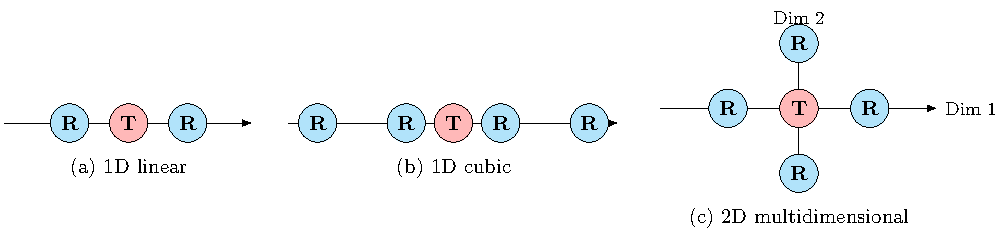
\includegraphics[width=\linewidth]{revised-fig/1-sz-qoz-predictors.pdf}
\caption{Representative interpolation stencils. $T$ denotes a prediction target and $R$ an available reconstructed reference. The layouts are schematic and not to scale.}
\label{fig:background:stencils}
\end{figure}

For multidimensional data, SZ3's basic interpolation scheme applies one-dimensional predictors in successive directional rounds. An axis permutation determines the order of these rounds among the rounds that share one spacing and is repeated as the spacing decreases. Changing the permutation changes which axis predicts each group of targets and which reconstructed values are available to later rounds. Sampled compression tests select the interpolation formula and axis ordering, but the coefficients within each formula remain fixed.

QoZ extends this design by selecting a linear or cubic interpolator and an axis order separately for every three consecutive rounds. Sampled prediction errors guide these selections, while the coefficients within each interpolator remain fixed.

QoZ further expands the predictor choices and optionally tunes them within individual blocks. Its choices include alternative cubic formulas and multidimensional interpolation that combines predictions along available axes. For example, another four-reference cubic formula uses coefficients $(-3,23,23,-3)/40$ at offsets $(-3h,-h,h,3h)$. These alternatives broaden the coefficient choices without searching arbitrary coefficient combinations. Direction-wise MSE is used to derive weights for combining predictions across axes. QoZ can also freeze a dimension, avoiding interpolation along that axis when doing so improves compression.

QoZ additionally tunes the precision assigned to different rounds. Let $k=1$ index the finest three rounds and larger $k$ index each successively coarser three rounds. For the rounds with index $k$, it sets
\begin{equation}
\label{eq:background:round-bound}
\epsilon_k=\frac{\epsilon_{\mathrm{abs}}}{\min(\alpha^{k-1},\beta)},\qquad \alpha\geq1,\ \beta\geq1.
\end{equation}
Here, $\alpha$ controls how quickly the error bound tightens toward coarser rounds and $\beta$ caps this tightening. More accurate coarse-round references can improve later predictions. Trial compression on sampled data selects these settings according to the resulting compression ratio and reconstruction quality.

These mechanisms illustrate how prediction stencils, coefficients, directions, and quantization precision jointly affect compression. They provide the baseline for our study of predictor configurations and quantization-bin serialization order in the following sections.
